\documentclass{chi2009}
\usepackage{times}
\usepackage{url}
\usepackage{graphicx} % PNGs
\usepackage[ngerman,english]{babel}
\usepackage[utf8x]{inputenc}
\usepackage[T1]{fontenc}
\usepackage{listings} % for sourcecode
\usepackage{graphviz} % graphs
\usepackage{array} % tables
\usepackage{afterpage} % figures
\usepackage{float} % figures
\usepackage{wrapfig} % figures im fließtext
\include{multicolumn}
\usepackage{graphics}
\usepackage{color}
\usepackage[pdftex]{hyperref}
\hypersetup{%
pdftitle={SocioPath},
pdfauthor={Konstantin Haase, Tim Felgentreff, Johannes Wollert}
pdfkeywords={UI,HCI},
bookmarksnumbered,
pdfstartview={FitH},
colorlinks,
citecolor=black,
filecolor=black,
linkcolor=black,
urlcolor=black,
breaklinks=true,
}
\newcommand{\comment}[1]{}
\definecolor{Orange}{rgb}{1,0.5,0}
\newcommand{\todo}[1]{\textsf{\textbf{\textcolor{Orange}{[[#1]]}}}}

\pagenumbering{arabic}  % Arabic page numbers for submission.  Remove this line to eliminate page numbers for the camera ready copy

\begin{document}
% to make various LaTeX processors do the right thing with page size
\special{papersize=8.5in,11in}
\setlength{\paperheight}{11in}
\setlength{\paperwidth}{8.5in}
\setlength{\pdfpageheight}{\paperheight}
\setlength{\pdfpagewidth}{\paperwidth}

% use this command to override the default ACM copyright statement 
% (e.g. for preprints). Remove for camera ready copy.
\toappear{%
Final report \\
Introduction to HCI 2008/2009, Prof. Patrick Baudisch\\
Hasso Plattner Institute}

\newcommand{\trademark}{\texttrademark~}
\newcommand{\registered}{\textregistered~}

\title{SocioPath: Mobilizing the Social Web on the Path to a Diverse Society}
\numberofauthors{1}
\author{
  \alignauthor Konstantin Haase, Tim Felgentreff, Johannes Wollert\\
    \affaddr{Hasso-Plattner-Institute}\\
    \affaddr{Prof.-Dr.-Helmert-Str. 2-3}\\
    \affaddr{D-14482 Potsdam, Germany}\\
    \email{~\\ 	$\big\{$konstantin.haase,tim.felgentreff,johannes.wollert$\big\}$@student.hpi.uni-potsdam.de}
}
\maketitle
\nocite{*}
\begin{abstract}
  With the rise of the Web 2.0 social networking sites, our social interactions
have gained another facet. As with every social activity, confinement
to a lone computer session thins out the user-group considerably.
If the social web is 
to persists this cannot be the end of the story. Yet, broad use of social networks on-the-go 
with the help of
the increasingly popular smartphones is held back by the large form factor of 
those devices, and the fact that they are not specialized to perform this 
task. In this paper, we propose a tiny mobile device tailored to the needs 
of the social web user. In our user study, participants were able to access
their most wanted features more quickly and with less error compared to a 
regular smartphone with a web browser.

\end{abstract}
\category{H.5.2}{[Information Interfaces and Presentation]} User Interfaces, Input devices and strategies
\keywords{mobile devices, touch, input devices}

  %:= the shortest path between a commonly believed fact
%and the research question you are answering in your paper
%
%Example (Shift, CHI 2007)
%to save time for retrieving the stylus, users operate PDAs using touch
%finger tip size and occlusion make acquisition of small targets hard
% zooming does not fix that occlusion (see section “user test paper”)
% offset cursor solves the problem, but has three drawbacks
%we propose ‘Shift’. It solves the problem while avoiding the 3 drawbacks
%
%one paragraph for each logical step in that argument
%if you need more than, say, 6 paragraphs you are probably underestimating your audience and started too far back
%write in logical order, not in the chronological order in which you came up with it (this is not a diary)
%
\section{Introduction}
Social Web is the next logical extension to Mail and SMS to keep track of your associates. 
Social websites have gained much larger user bases than ``traditional'' web communities and demand
for new ways of access to the communities is high.
Traditionally, 
anything web-related was performed at a computer and only recently, with the wide-spread adoption of 
smartphones, the desire to use such networks ubiquitously emerged. Let's see how this is done today:
\begin{itemize}
  \item %
    Users usually 
    use the web browser of their smartphone system. This is the obvious solution for the inexperienced,
    and it is guaranteed to work with their social network of choice.
  \item Even with clever zooming techniques, the small screen is unsuitable for feature-packed sites such as Facebook\registered. 
    This alienates users. Still, they will likely not give up social networking, but rather look for a new 
    way of using it on-the-go
  \item Persistent users will soon find specialized apps for example on the Android\trademark platform or for the 
    Palm\registered Pre, however, 
    those apps still have to be started each time. Such delay, now matter how small, may offset users from doing what they were 
    trying to do completely, as users generally do not see the point of waiting 10 seconds for an application to start 
    only to see they do not have any new messages in their inbox.
\end{itemize}
To resolve those issues,we propose a specialized, small and unobtrusive device tailored towards a 
single purpose: to access the 
most used features of social networks in a consistent manner without delay or other 
inconvenience. We want social networking to
become the natural daily experience its users wanted it to be all along.
\begin{figure}[h]
  \begin{center}
    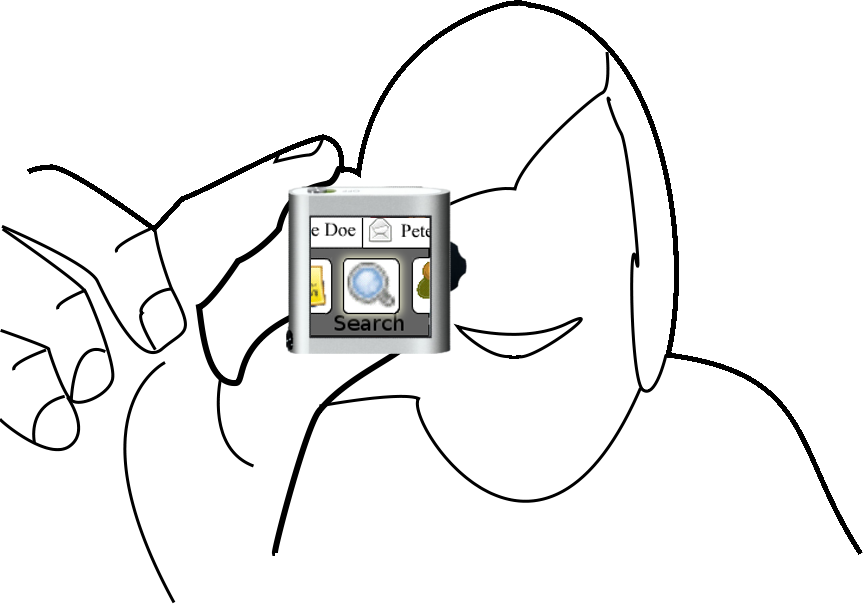
\includegraphics[width=0.8\linewidth]{imgs/main.png}
  \end{center}
  \caption{The SocioPath Device in Context}
  \label{fig:main}
\end{figure}

  %why readers should care (not why you wrote it)
%
\paragraph{Motivation}

  % The most comprehensible way of showing your final design 
% (and why it matters) is to give a walkthrough of the key task.
%
% make a sequence of screenshots. Crop and add callouts if necessary 
% to reveal detail such as text in the UI.
%
% Start by showing the final design, then explain why you did it
% 
% keep intro and walkthrough short by explaining only 
% (this is not literature class. Don’t give in to “but if I say 
% everything right away, why would attendees/readers continue to 
% pay attention?”
%
\clearpage
\subsection{Walkthrough - Photo Browsing}
%
As we found out during User Studies and the Contextual Inquiry, one of the most widely used features of social websites is picture browsing.
That is why we provide corresponding functionality to perform this task.

\begin{figure}[h]
  \begin{center}
    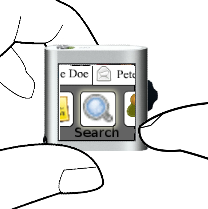
\includegraphics[width=0.6\linewidth]{imgs/wt1.png}
  \end{center}
  \caption{The Main Screen with Vertical Scrolling, Thumb-sized Icons}
  \label{fig:wt1}
\end{figure}
%
As shown in Fig. \ref{fig:wt1}, every action performed by a user starts in the Main Menu. There is a ticker on top of it, covering the latest news from your friends. Scrolling through the menu is done by swiping gestures or the thumbwheel.
To browse the pictures of a person, we have to find the person first. That is why the search function is selected, simply by tapping on the icon.

\begin{figure}[h]
  \begin{center}
    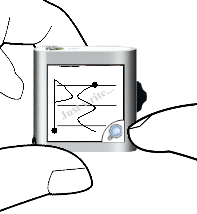
\includegraphics[width=0.6\linewidth]{imgs/wt2.png}
  \end{center}
  \caption{The Writing Recognition Offers Visual Feedback}
  \label{fig:wt2}
\end{figure}
%
To proceed, the name of the person is typed in, as shown in Fig. \ref{fig:wt2}.
\\
\begin{figure}[h]
  \begin{center}
    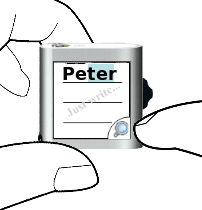
\includegraphics[width=0.6\linewidth]{imgs/wt3.png}
  \end{center}
  \caption{Type-Ahead for Quick Access}
  \label{fig:wt3}
\end{figure}
%
Auto-completion features are used to provide easier and effortless text input (Fig. \ref{fig:wt3}) which is crucial on very small screens.\\
\begin{figure}[h]
  \begin{center}
    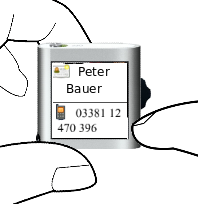
\includegraphics[width=0.6\linewidth]{imgs/wt4.png}
  \end{center}
  \caption{A Vertically Scrolling Profile View}
  \label{fig:wt4}
\end{figure}
%
The Profile View on our device, as depicted in Fig. \ref{fig:wt4}, shows a set of the most important information on the respective person. Again, scrolling through the menu is done by gestures or the thumbwheel.\\
%
\begin{figure}[h!]
  \begin{center}
    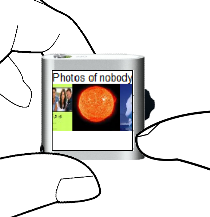
\includegraphics[width=0.6\linewidth]{imgs/wt5.png}
  \end{center}
  \caption{Viewing Albums of a User}
  \label{fig:wt5}
\end{figure}
%
Concerning interaction, viewing photo albums (Fig. \ref{fig:wt5}) is just the same as browsing the Main Menu. This ensures a consistent look-and-feel throughout our user interface.

\begin{figure}[h]
  \begin{center}
    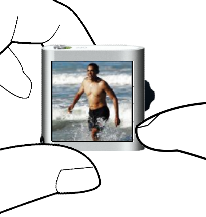
\includegraphics[width=0.6\linewidth]{imgs/wt6.png}
  \end{center}
  \caption{A Fullscreen Photo View}
  \label{fig:wt6}
\end{figure}
%
Concerning the limitations of a Euro-sized screen, we decided that the actual Photo View has to be done in Fullscreen mode, as displayed in Fig. \ref{fig:wt6}. That way, pictures remain recognizable within reasonable distances.
%

  % be respectful with people you reference
% people you reference (and committee members) are likely to be reviewers
%
% you need to say how you are different from the 1-3 key pieces of 
% related work; for all others just write “xx did yy.”
%
% Mention limitations and drawbacks in a sentence, not a paragraph
%
\subsection{Related Work}

There is the Palm Pre, the T-Mobile G1 (possibly even G2) and something we like to call ``MacBook pro''.
However, all of the mentioned produces (except for the G2, maybe, but that remains unknown), are really second class
compared to the SocioPath and actually not worth mentioning. Our main advantage: The SocioPath is smaller.
But this goes hand in hand with our biggest drawback: Our screen is very tiny and you might have to get real close
when watching photos.
  % explains why yours is the best possible design
% helps others avoid dead ends
%
% your final design is typically the result of exploring a tree
%
% keep intro and walkthrough short by explaining only 
% in a separate design section mention dead ends
% do not drill deeper into dead ends though
%
\section{Design}
%
To create our device we used five techniques 
to observe the target groups needs and funnel those 
into an ever more refined design. 
\begin{description}
  \item[User Study] We never intended to win new customers to 
    the social-web idea, instead we focused on customers already 
    using services like Twitter\trademark or Facebook\registered. 
    We believe that social networks are the Web 2.0 killer application. 
    Customers are flocking to them at the same time, mobile devices
    become increasingly more popular, so demand for a union of 
    those has risen considerably, as we found out during our preliminary 
    user study.
  \item[Contextual Inquiry]
    During our contextual inquiry we were able to identify some stereotypical 
    target users and created common task descriptions those users would 
    attempt most often. While the user focus seems to differ largely, ranging 
    from staying in touch using messages to just using them as an automtic 
    birthday reminder, all of them used the messaging functionality and 
    shared photos with their friends.
  \item[Task Analysis]
  \item[Functionality and Design]
  \item[Usability Flaws and Paper Prototyping]
  \item[Interactive Prototype]
\end{description}

  \section{Conclusions}
We managed to build a functional and flexible FrozenBubble clone for Morphic,
but given our time constraints, not all features we would have liked to implement
made it into the final version. Especially a working network multiplayer mode would
have been quite delightful. It is possible however to play a local multiplayer mode,
limited in use only by the self-blocking keypress messages provided by morphic.

\section*{Acknowledgements}
We are indebted to the developers of Frozen Bubble for allowing us to release 
our clone with the name and graphics of the original game under the MIT 
license. We also thank Professor Hirschfeld, Tobias Pape and Michael Perscheid for 
their advice.


\bibliographystyle{abbrv}
\bibliography{ui}
\end{document}
